% 中文节标题：实验
% 中文：阻止实验内容回漂到方法节。
\FloatBarrier
\section{Experiments}
\label{sec:experiments}

% 中文：在实验设置之前引入核心定性结果。
\begin{figure*}[t]
  \centering
  % 从完整可编辑七方法图中无损裁取正文关键方法列；完整版本见附录。
  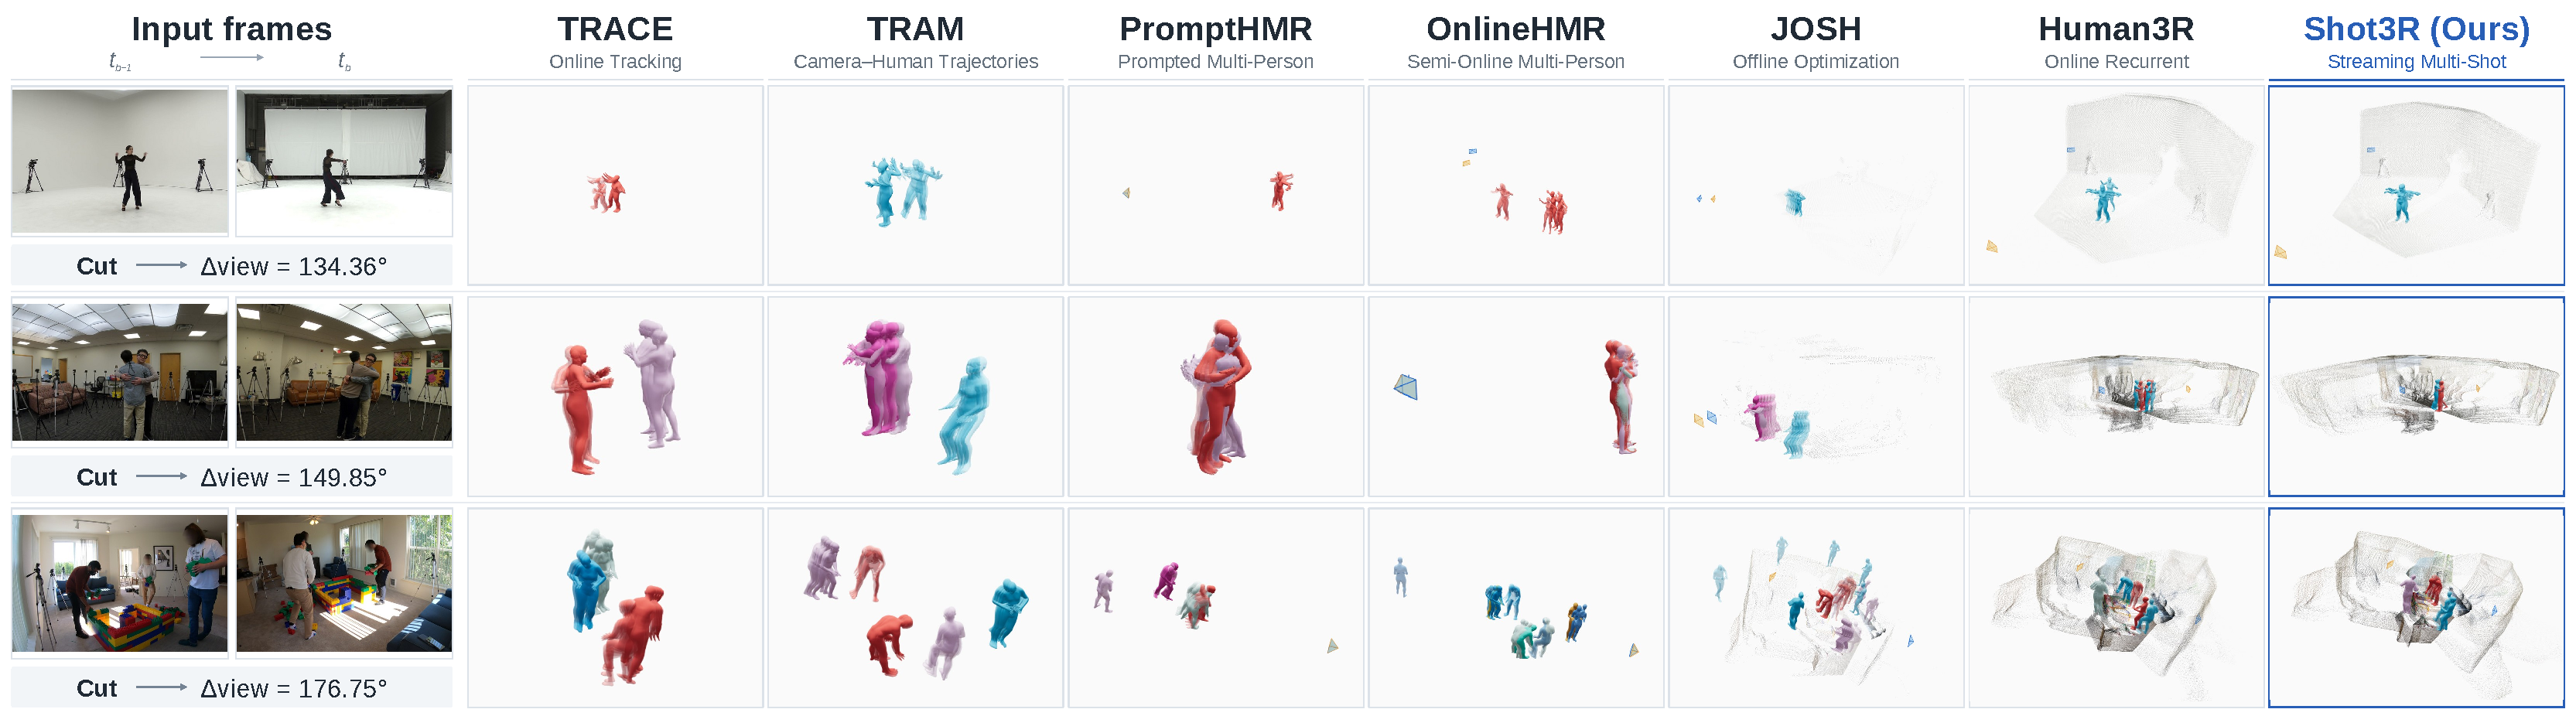
\includegraphics[height=0.415\textwidth,trim=0pt 0pt 1315pt 0pt,clip]{figures/Shot3R_qualitative_comparison.pdf}\hspace{-1.2mm}%
  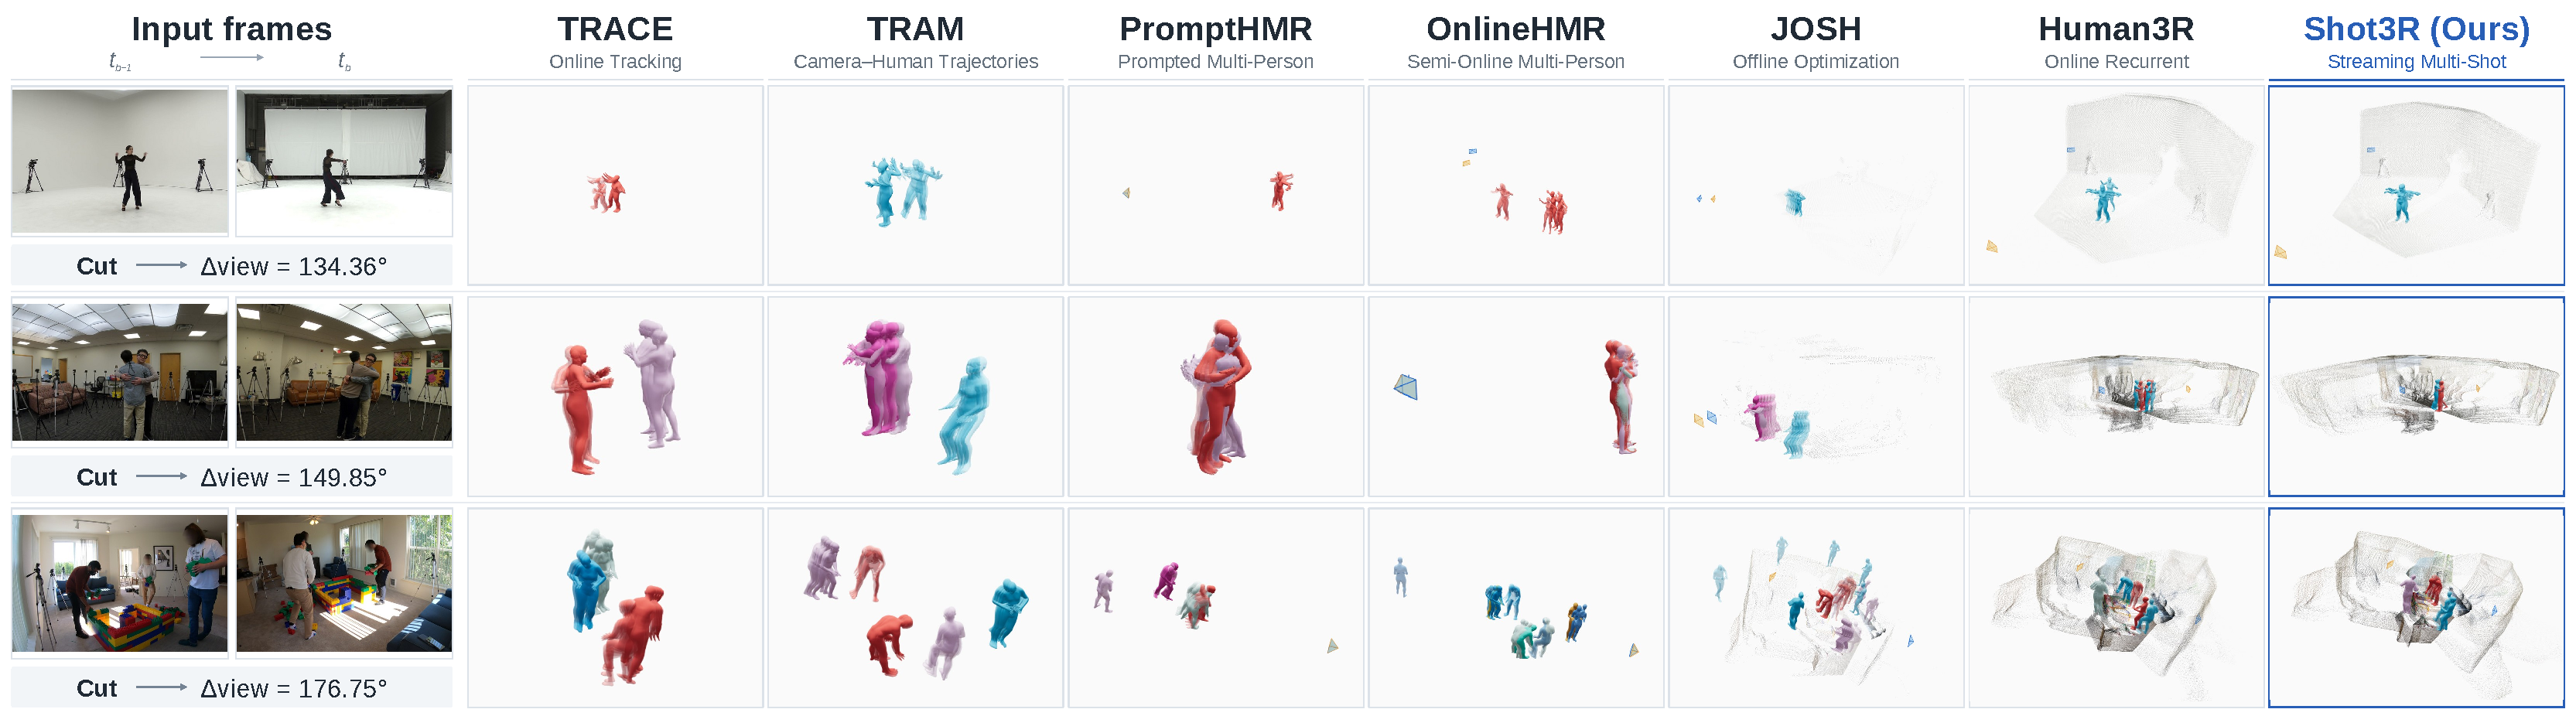
\includegraphics[height=0.415\textwidth,trim=845pt 0pt 560pt 0pt,clip]{figures/Shot3R_qualitative_comparison.pdf}\hspace{-1.2mm}%
  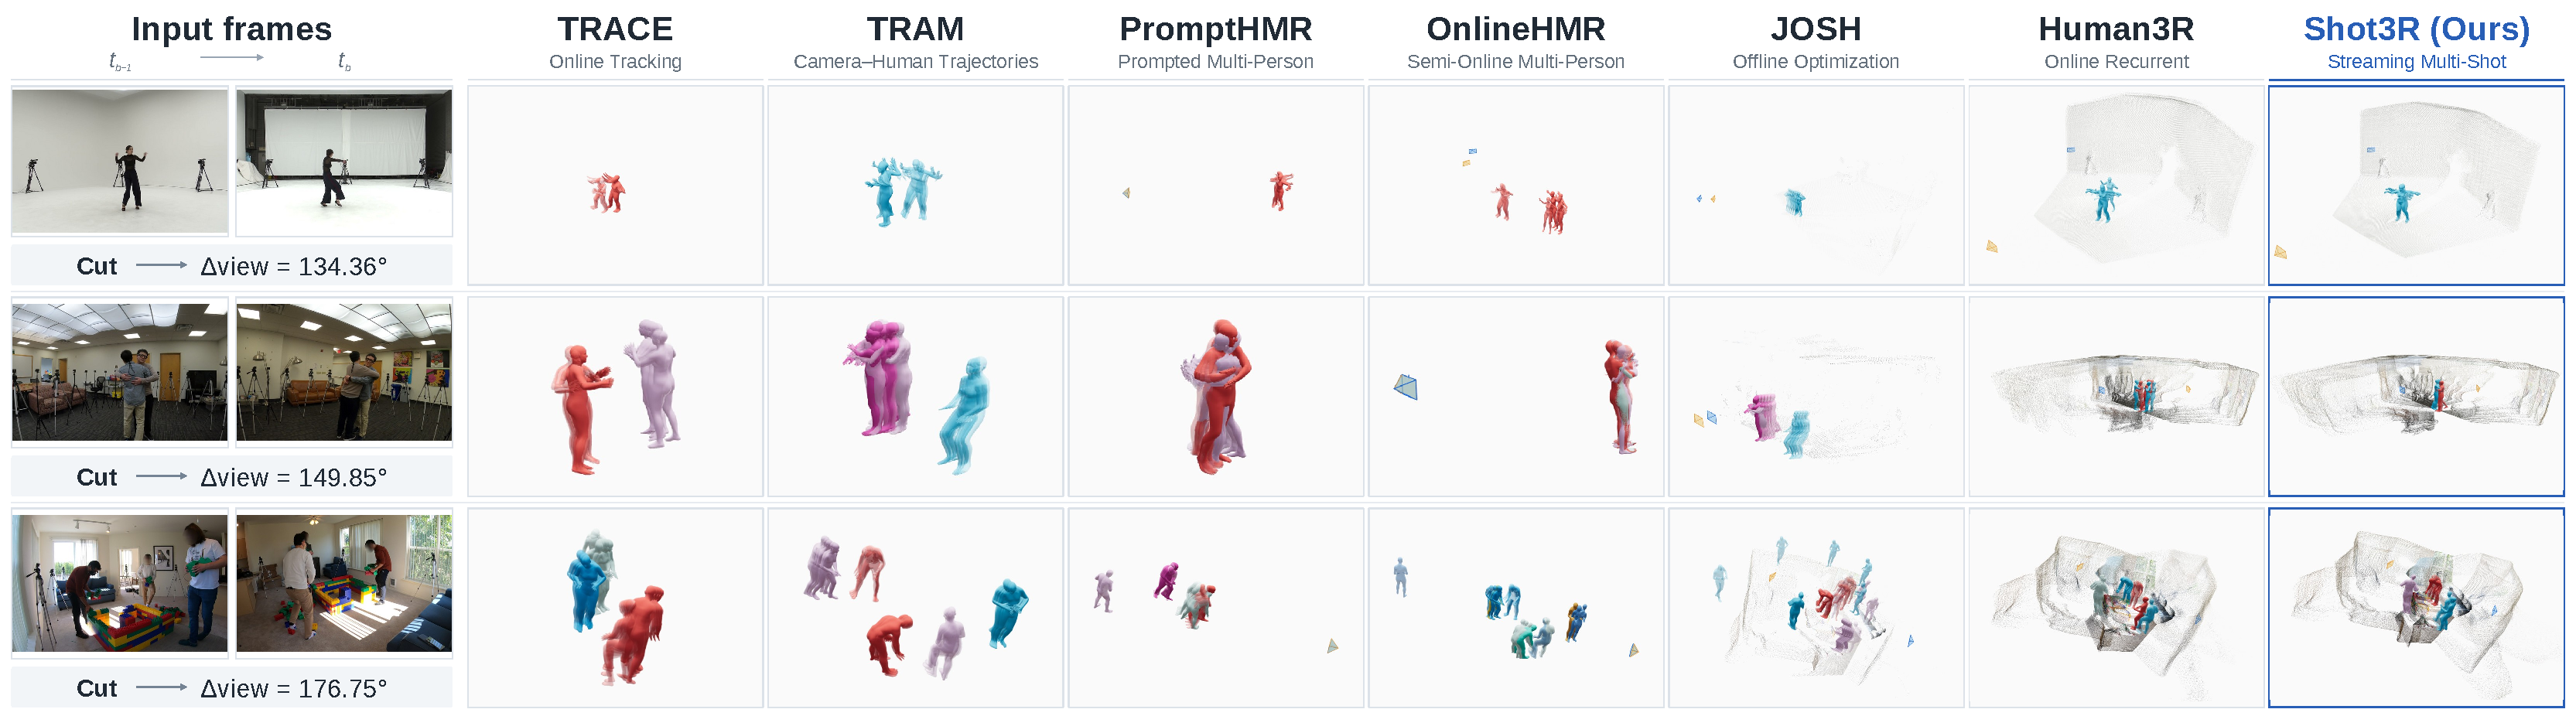
\includegraphics[height=0.415\textwidth,trim=1034pt 0pt 374pt 0pt,clip]{figures/Shot3R_qualitative_comparison.pdf}\hspace{-1.2mm}%
  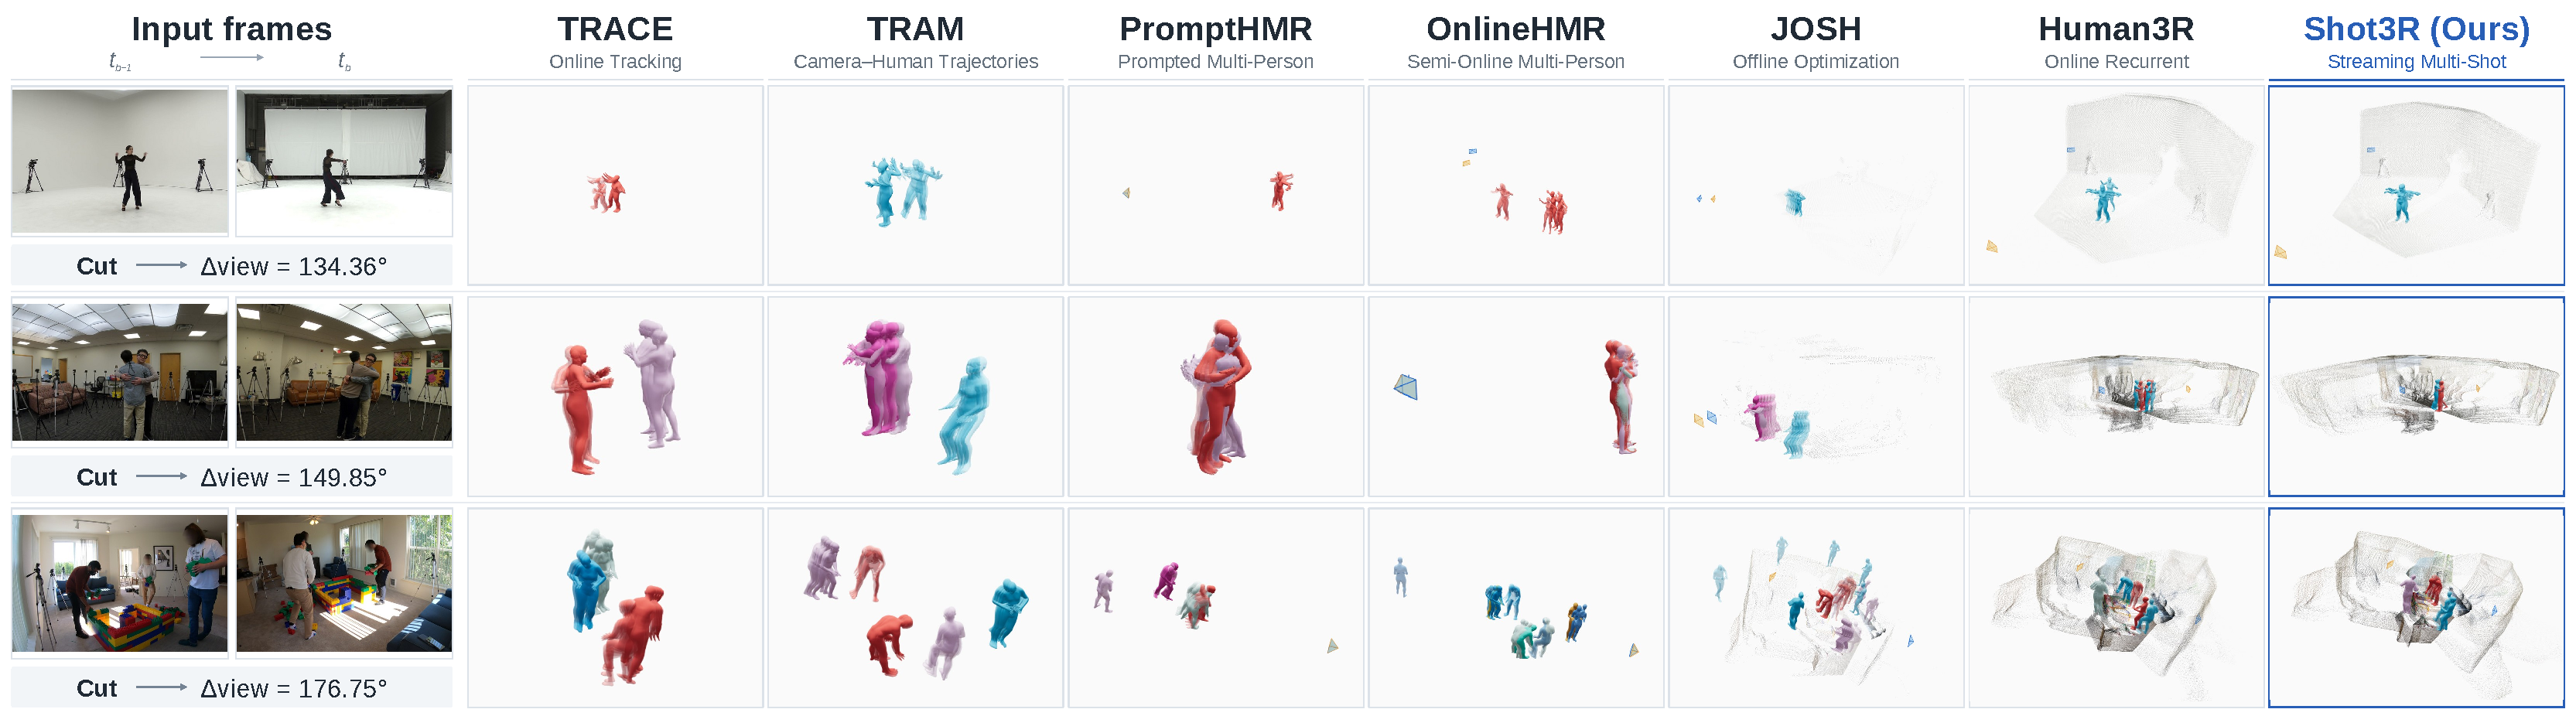
\includegraphics[height=0.415\textwidth,trim=1220pt 0pt 188pt 0pt,clip]{figures/Shot3R_qualitative_comparison.pdf}\hspace{-1.2mm}%
  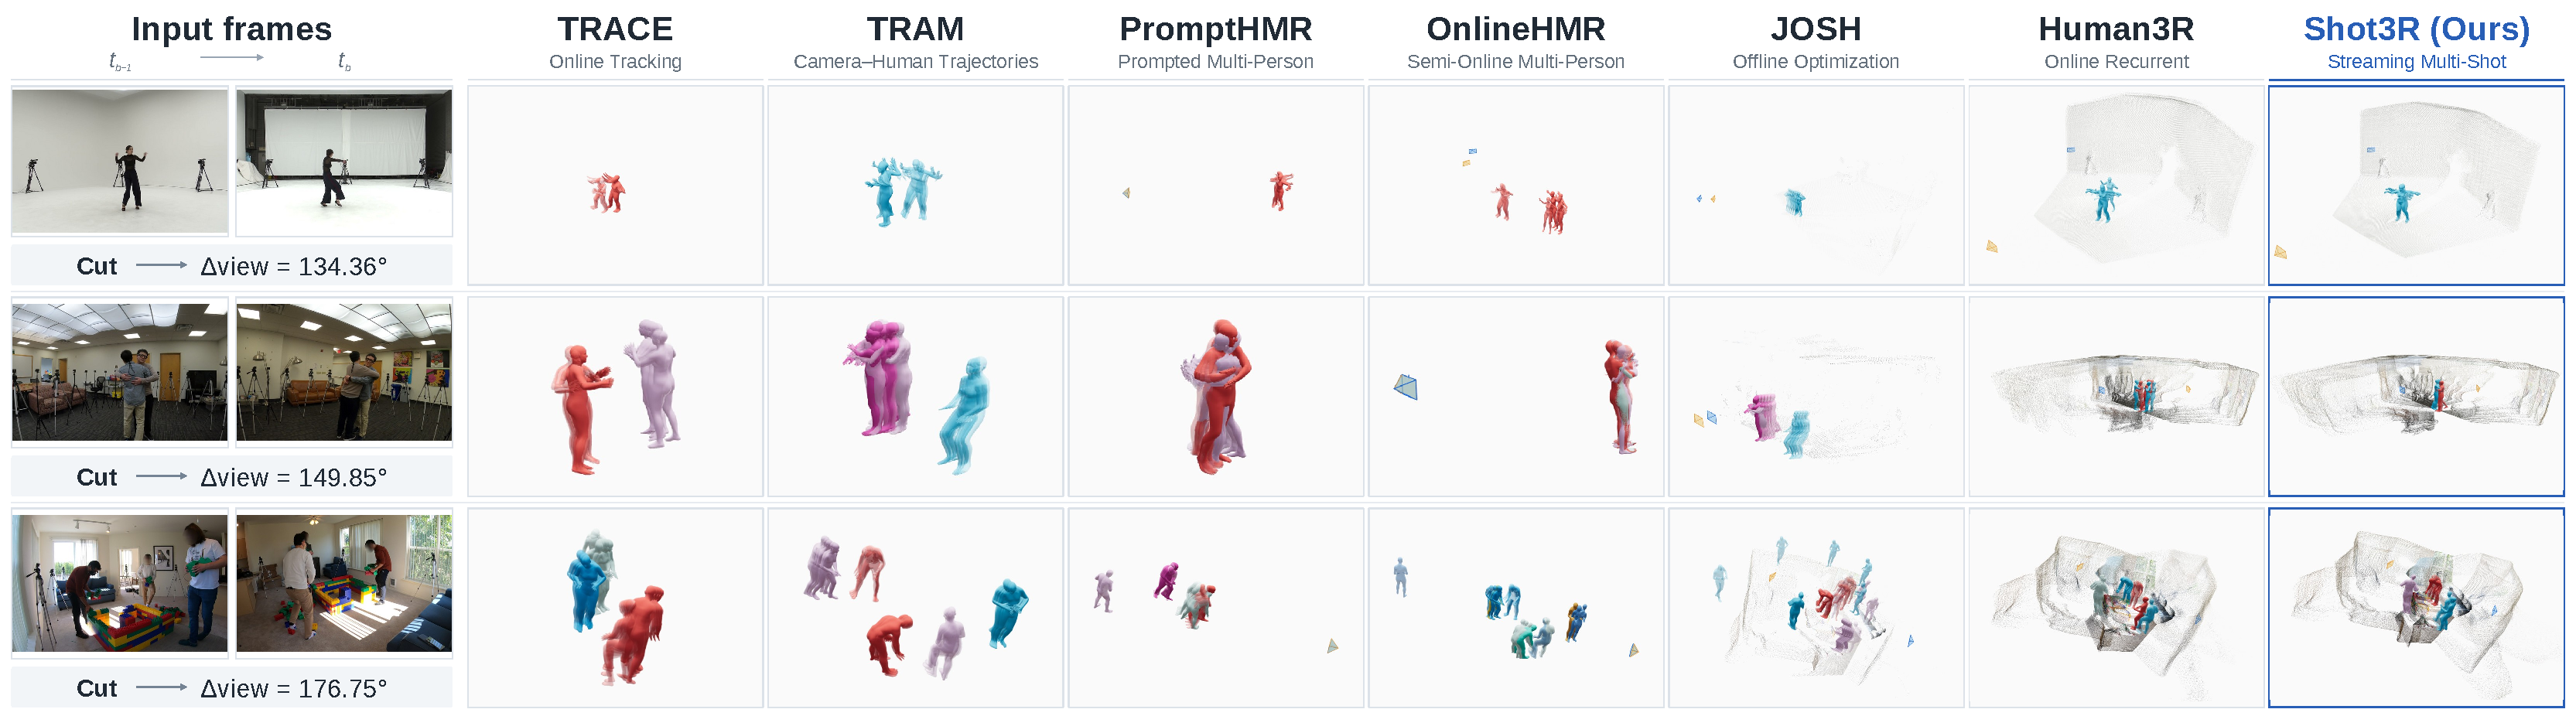
\includegraphics[height=0.415\textwidth,trim=1407pt 0pt 0pt 0pt,clip]{figures/Shot3R_qualitative_comparison.pdf}
  % 中文图注：跨镜头切换的关键定性比较。每一行首先展示切换前后的输入，随后是半在线、离线、在线递归基线与本文结果。
  % 三个视角变化从上到下为134.36、149.85和176.75度。Shot3R维持更连贯的相机—人体布局；各方法可用的场景输出一并显示。
  \caption{\textbf{Key qualitative comparisons across shot transitions.}
  Inputs before and after each transition are followed by OnlineHMR, JOSH,
  \humanthree{}, and \method{}. Viewpoint changes are $134.36^\circ$,
  $149.85^\circ$, and $176.75^\circ$ from top to bottom. \method{} maintains a
  more coherent camera--human layout; scene geometry is shown where available.
  The complete seven-method view is in Appendix~\ref{app:qualitative-full}.}
  \label{fig:qualitative-comparison}
\end{figure*}


% 中文小节标题：实验设置
\subsection{Experimental Setup}

% 中文段落标题：对比方法。
% 中文：我们采用公开发布的Human3R检查点作为主要受控基线。Human3R和Shot3R接收相同的顺序RGB帧，
% 并使用相同的预处理和评测流程；主要区别是Human3R持续传播递归状态，而Shot3R在检测到镜头切换时，
% 使用历史条件对齐并重新初始化递归过程。我们还评测OnlineHMR、TRACE、PromptHMR和JOSH的官方实现，
% 并将TRAM纳入统一计时。主表按时间信息访问方式对方法分组，并标明其是否显式处理镜头切换。
% HumanMM和Multi-THuMBS作为文献背景讨论，但由于完整代码、权重和评测配置尚未公开，不纳入定量比较。
\paragraph{Baselines.}
We use the publicly released \humanthree{} checkpoint as our primary
controlled baseline. \humanthree{} and \method{} receive the same ordered RGB
frames, preprocessing, and evaluation; the principal difference is that
\humanthree{} propagates its recurrent state continuously, whereas \method{}
handles each detected transition through history-conditioned alignment and
reinitialized recurrence. We additionally evaluate the official
implementations of OnlineHMR, TRACE, PromptHMR, and JOSH, and include TRAM in
the standardized timing study
~\citep{zhao2026onlinehmr,sun2023trace,wang2025prompthmr,liu2026josh,wang2024tram}.
Table~\ref{tab:multi-person} groups methods by temporal access and marks
explicit transition handling; preprocessing and output scope are reported in
Appendix~\ref{app:protocol}. HumanMM and Multi-THuMBS are included as
literature context but not in the quantitative comparison because their
complete code, model weights, and evaluation configurations are not publicly
available.

% 中文段落标题：数据集与评价指标。
% 中文：我们基于EgoBody、EgoHumans和Harmony4D构建顺序多镜头输入，将其同步采集转换为依次输入、
% 而非同时输入的单目镜头，分别得到129、90和88个固定评测样例。EgoBody支持镜头边界机制的受控分析，
% EgoHumans包含显著视角变化，Harmony4D则提供密集多人交互和重复镜头切换评测。
% W-MPJPE使用最早有效观测确定并固定Sim(3)对齐，对镜头间位置偏移敏感；WA-MPJPE使用全部有效观测对齐。
% 我们还报告相机轨迹误差、衡量跨镜头身份连续性的IDF1，以及反映缺失预测的Coverage。
\paragraph{Datasets and metrics.}
We construct sequential multi-shot inputs from EgoBody, EgoHumans, and
Harmony4D~\citep{zhang2022egobody,khirodkar2023egohumans,khirodkar2024harmony4d}.
Their synchronized recordings are converted into monocular shots presented
successively rather than simultaneously, yielding 129, 90, and 88 fixed
evaluation cases, respectively. EgoBody supports controlled analysis of the
boundary mechanism, EgoHumans contains substantial viewpoint changes, and
Harmony4D provides crowded multi-person interactions and repeated-transition
evaluations. W-MPJPE (W) fixes a Sim(3) alignment using the earliest valid
observations and is therefore sensitive to cross-shot displacement, whereas
WA-MPJPE (WA) aligns all valid observations. We further report camera
trajectory error, IDF1 for cross-shot identity continuity
~\citep{ristani2016performance}, and Coverage to account for missing
predictions. Metric definitions and aggregation protocols are detailed in
Appendix~\ref{app:protocol}.

% 中文段落标题：实现细节。
% 中文：Shot3R仅在AvatarReX和THuman上训练，两者均不属于评测基准。我们选择性优化19.62M个参数，
% 占完整1.208B参数模型的1.63%。可训练参数包括镜头边界对齐组件与低秩适配参数，其余预训练主干保持冻结。
% 该设计将适配集中于镜头边界处当前观测与递归历史的交互，同时保留预训练的镜头内重建先验。
% 所有基准使用同一检查点和推理配置，不进行针对数据集或单个视频的优化。
\paragraph{Implementation details.}
\method{} is trained exclusively on AvatarReX and THuman, which are disjoint
from all evaluation benchmarks. We selectively optimize 19.62M parameters,
corresponding to 1.63\% of the complete 1.208B-parameter model. These
trainable parameters comprise the shot-boundary alignment components and
low-rank adapters, while the original pretrained backbone remains frozen.
This confines adaptation to the interaction between current observations and
recurrent history at shot boundaries while preserving the pretrained
within-shot reconstruction prior. All benchmarks use a single checkpoint and
inference configuration, without dataset- or video-specific optimization.
Appendix~\ref{app:implementation} provides the training-data composition,
optimization schedule, parameter breakdown, hardware configuration, and
convergence curves.

% 中文小节标题：多镜头多人体重建
\subsection{Multi-Shot Multi-Person Reconstruction}
\label{sec:main-results}

% 中文：主结果表在逻辑上归入4.2。
\begin{table*}[t]
  \centering
  % 中文图注：EgoBody和EgoHumans上的多镜头多人体重建。正文保留所有已完成准确率评测的方法，按时间访问方式分组；Transition表示是否显式处理镜头切换。
  \caption{Comparison on the EgoBody and EgoHumans multi-shot multi-person reconstruction protocols.}
  \label{tab:multi-person}
  \footnotesize
  \setlength{\tabcolsep}{2.7pt}
  \renewcommand{\arraystretch}{1.04}
  \newcommand{\evaln}[2]{#1\textsuperscript{\tiny #2}}
  \resizebox{\textwidth}{!}{%
  \begin{tabular}{llc rrrrr rrrrr}
    \toprule
    & & & \multicolumn{5}{c}{EgoBody ($N=129$)} & \multicolumn{5}{c}{EgoHumans ($N=90$)} \\
    \cmidrule(lr){4-8}\cmidrule(lr){9-13}
    Category & Method & Transition & W $\downarrow$ & WA $\downarrow$ & ATE $\downarrow$ & IDF1 $\uparrow$ & Cov. $\uparrow$ & W $\downarrow$ & WA $\downarrow$ & ATE $\downarrow$ & IDF1 $\uparrow$ & Cov. $\uparrow$ \\
    \midrule
    \multirow{2}{*}{Offline}
      & PromptHMR (SPEC) & \xmark & \evaln{741.4}{64} & \evaln{336.1}{87} & -- & 0.195 & 0.202 & \evaln{1193.3}{17} & \evaln{487.7}{25} & -- & 0.061 & 0.062 \\
      & JOSH & \xmark & \evaln{399.6}{127} & \evaln{322.9}{127} & \evaln{0.087}{127} & 0.973 & 0.980 & \evaln{1410.7}{77} & \evaln{481.3}{77} & \evaln{1.755}{87} & \textbf{0.616} & \textbf{0.686} \\
    \midrule
    Semi-online
      & OnlineHMR & \xmark & \evaln{961.2}{97} & \evaln{418.1}{97} & \evaln{0.259}{129} & 0.375 & 0.424 & \evaln{1311.7}{50} & \evaln{405.5}{50} & \evaln{3.869}{87} & 0.142 & 0.211 \\
    \midrule
    \multirow{3}{*}{Online}
      & TRACE & \xmark & \evaln{576.4}{22} & \evaln{276.4}{35} & -- & 0.036 & 0.035 & \evaln{2464.6}{43} & \evaln{749.5}{59} & -- & 0.070 & 0.072 \\
      & \humanthree{} & \xmark & 321.1 & 233.4 & 0.124 & 0.870 & \textbf{0.981} & 1005.1 & 365.7 & 1.673 & 0.471 & \underline{0.639} \\
      & \textbf{\method{}} & \cmark & \textbf{258.8} & \textbf{201.7} & \textbf{0.016} & \textbf{0.985} & \textbf{0.981} & \textbf{866.8} & \textbf{336.9} & \textbf{1.423} & \underline{0.571} & 0.616 \\
    \bottomrule
  \end{tabular}%
  }
  \vspace{0.5mm}

  % 中文表注：Transition表示显式处理镜头切换。W/WA单位为毫米；EgoBody的ATE-Sim3和EgoHumans的ATE-SE3单位为米。上标为条件几何指标的可评测视频数；IDF1和Coverage使用完整固定分母。不同支持数上的条件几何均值不构成统一排名。
  \parbox{0.98\textwidth}{\scriptsize Transition denotes explicit shot-transition handling. W/WA are in mm and ATE in m (Sim(3) on EgoBody; SE(3) on EgoHumans). Superscripts give the number of evaluable streams for conditional geometry metrics; IDF1 and Coverage use the complete predefined protocol. Geometry means computed on different supports do not constitute a common ranking.}
\end{table*}


% 中文：主表报告EgoBody和EgoHumans，Harmony4D完整结果见附录。在主要受控比较中，Shot3R相对Human3R
% 在三个数据集上均改善WA、相机误差和IDF1；W在EgoBody和EgoHumans上改善，在Harmony4D上略有增加。
% EgoBody的局部姿态与网格精度基本不变，说明主要收益来自统一坐标系中的空间关系、相机轨迹与身份连续性，
% 而不是重新学习镜头内部的人体重建。公开系统比较与受控机制比较承担不同作用，并需结合有效样本支持理解条件误差。
Table~\ref{tab:multi-person} reports EgoBody and EgoHumans, with the complete
Harmony4D comparison in Appendix~\ref{app:full-results}. In the controlled
comparison with \humanthree{}, \method{} improves WA, camera error, and IDF1
on all three datasets; W improves on EgoBody and EgoHumans and increases
modestly on Harmony4D. On EgoBody, W/WA decreases from 321.1/233.4 to
258.8/201.7\,mm, ATE from 0.124 to 0.016\,m, and IDF1 rises from 0.870 to
0.985 at unchanged 0.981 Coverage. Local pose and mesh accuracy remain
essentially unchanged (Appendix Table~\ref{tab:supp-egobody-local}), indicating
that the gains arise primarily from spatial placement in the common frame,
camera estimation, and identity continuity rather than relearning within-shot
body reconstruction. The public-system comparison provides complementary
evidence: on shared valid inputs, \method{} lowers human and camera errors
relative to OnlineHMR and raises IDF1 and Coverage over complete streams; it
also yields lower W/WA/ATE than the offline JOSH pipeline on cases evaluable by
both methods across all three datasets, without future-frame access. Because
TRACE and PromptHMR return evaluable geometry for only subsets of EgoBody,
their conditional errors must be interpreted together with valid support;
complete paired comparisons and failure records are provided in the appendix.

% 中文：当镜头间视角差增大时收益更加明显。按数据集等权汇总，全部视角的W降低9.5%，大视角子集降低19.1%；
% EgoBody极端视角中W降低29.9%，IDF1从0.758提升至0.983。定性图展示134.36、149.85和176.75度切换，
% Shot3R在明显的视角和外观变化后仍维持更连贯的相机—人体布局。完整分层结果和连续角度分析见附录。
The advantage becomes more pronounced as the inter-shot viewpoint change
increases. With equal weight per dataset, \method{} reduces W-MPJPE by 9.5\%
over all viewpoints and by 19.1\% on the predefined large-viewpoint subsets.
On extreme-view EgoBody, W-MPJPE decreases by 29.9\%, while IDF1 rises from
0.758 to 0.983. Figure~\ref{fig:qualitative-comparison} further shows
transitions of $134.36^\circ$, $149.85^\circ$, and $176.75^\circ$: despite
pronounced viewpoint and appearance changes, \method{} retains a more
coherent camera--human layout. Figure~\ref{fig:angle-strata} and the appendix
report the complete viewpoint strata and continuous-angle analysis.

\begin{figure*}[t]
  \centering
  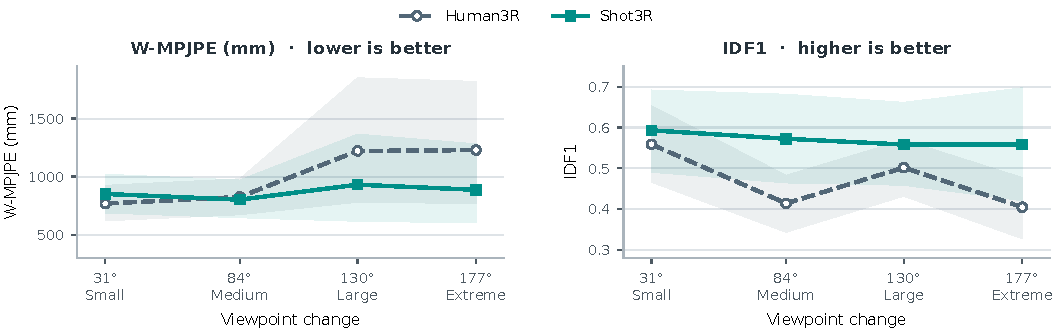
\includegraphics[width=0.82\textwidth]{figures/egohumans_angle_strata.pdf}
  % 中文图注：EgoHumans 中随镜头视角变化的重建和身份表现。曲线给出四个固定视角区间内的
  % W-MPJPE 和 IDF1 绝对值，阴影为以 capture 为单位 bootstrap 得到的 95% 置信区间。
  % Shot3R 在全部区间均获得更高 IDF1，并在 130° 与 177° 的大视角区间明显降低 W-MPJPE。
  \caption{\textbf{Viewpoint response on EgoHumans.} Curves report absolute
  W-MPJPE and IDF1 in four fixed angle strata; bands are capture-bootstrap 95\%
  confidence intervals. \method{} improves IDF1 throughout, with the clearest
  W-MPJPE reductions at $130^\circ$ and $177^\circ$.}
  \label{fig:angle-strata}
\end{figure*}


% 中文小节标题：分析与消融实验
\subsection{Analysis and Ablation Studies}
\label{sec:ablation}

% 中文：使用同一原始Human3R检查点、相同切换后RGB和静态物理相机，比较旧状态延续与重新初始化。
% 两条轨迹均锚定到新镜头首个预测以消除固定坐标变换。后续16帧中，状态延续产生1.124米/14.58度漂移，
% 重新初始化仅产生0.026米/0.20度漂移，且后者在全部27个capture上均更低。
% 因此，旧状态延续引起的是新镜头内随时间变化的漂移，而不仅是一个固定坐标偏移。
We first isolate the effect of state carry-over using the same original
\humanthree{} checkpoint on identical post-transition RGB in 90 EgoHumans
cases captured by a static physical camera, without any \method{} component.
Both camera trajectories are anchored to their first new-shot prediction,
removing any fixed coordinate transform. Over the next 16 frames, carrying
the old state produces 1.124\,m/$14.58^\circ$ translation/rotation drift,
compared with 0.026\,m/$0.20^\circ$ after reinitialization; the latter is lower
on all 27 captures. Old-state carry-over therefore induces time-varying
within-shot drift, not merely a fixed coordinate offset. Confidence intervals,
window-length controls, and paired tests are reported in
Appendix~\ref{app:egohumans-state-isolation}.

\begin{figure*}[t]
  \centering
  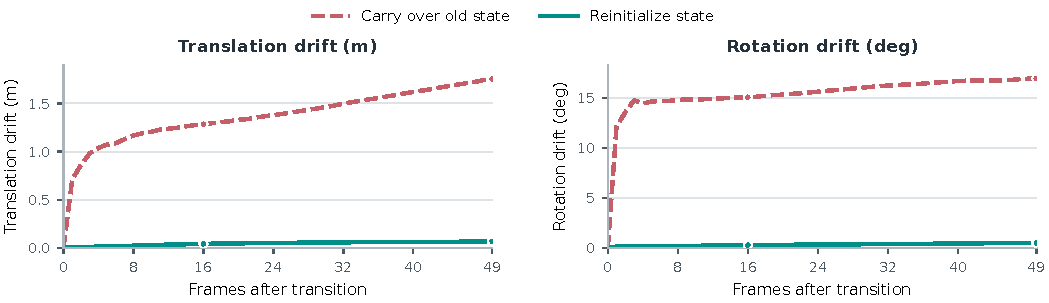
\includegraphics[width=0.80\textwidth]{figures/state_carryover_drift.pdf}
  % 中文图注：静态相机采集上的旧状态延续控制。相同的未修改Human3R检查点处理相同的新镜头RGB，且不使用Shot3R模块；
  % 首帧锚定消除固定坐标变换。旧状态延续产生镜头内漂移，而重新初始化保持稳定。
  \caption{\textbf{Old-state carry-over causes within-shot camera drift.}
  On static-camera captures, the same unmodified \humanthree{} checkpoint
  processes identical new-shot RGB with no \method{} component. First-prediction
  anchoring removes any fixed transform; carry-over then drifts while
  reinitialization remains stable.}
  \label{fig:state-drift}
\end{figure*}

\begin{table*}[t]
  \centering
  % 中文图注：EgoBody 上的对齐—状态传播 2×2 受控实验及完整 Shot3R。
  % 执行边界操作的三个受控设置使用标注镜头边界，Human3R 不读取边界，完整 Shot3R 使用在线检测边界。
  \caption{Alignment--state-propagation $2\!\times\!2$ control and the complete
  \method{} on EgoBody.}
  \label{tab:mechanism-evidence}
  \scriptsize
  \setlength{\tabcolsep}{2.0pt}
  % 中文列名：设置；边界信号；历史条件对齐；后续传播状态；跨镜头人物关联；
  % W-MPJPE（毫米）；WA-MPJPE（毫米）；ATE（米）；IDF1。
  \resizebox{\textwidth}{!}{%
  \begin{tabular}{lccccrrrr}
    \toprule
    \multirow{2}{*}{Configuration} & \multirow{2}{*}{Boundary cue} &
    \multicolumn{3}{c}{Shot-transition operation} &
    \multicolumn{4}{c}{EgoBody metrics} \\
    \cmidrule(lr){3-5}\cmidrule(lr){6-9}
    & & Alignment & \shortstack{Propagated\\state} & Association &
    W (mm) $\downarrow$ & WA (mm) $\downarrow$ & ATE (m) $\downarrow$ & IDF1 $\uparrow$ \\
    \midrule
    \humanthree{} & --- & \xmark & Continued & \xmark &
      321.1 & 233.4 & 0.124 & 0.870 \\
    State reinitialization & Annotated & \xmark & Reinitialized & \xmark &
      752.6 & 589.4 & 1.141 & 0.834 \\
    Alignment + continued state & Annotated & \cmark & Continued & \xmark &
      293.3 & 227.3 & 0.082 & 0.868 \\
    \shortstack[l]{Alignment +\\reinitialized state} & Annotated & \cmark & Reinitialized & \xmark &
      352.8 & 267.7 & 0.017 & 0.834 \\
    \textbf{\method{}} & Detected & \cmark & Reinitialized & \cmark &
      \textbf{258.8} & \textbf{201.7} & \textbf{0.016} & \textbf{0.985} \\
    \bottomrule
  \end{tabular}%
  }
  \vspace{1pt}

  % 中文表下注释：标注边界用于三个执行边界操作的受控设置；Human3R 不使用边界信号。
  % 两个已对齐设置关闭显式人物关联与人物引导的共享平移，只改变对齐后传播的状态。
  \parbox{0.96\textwidth}{\scriptsize Annotated boundaries are used only by
  the controlled configurations; \humanthree{} receives no boundary cue. The
  two aligned controls disable association and person-guided translation, so
  only the state propagated after alignment changes.}
\end{table*}


% 中文：表格将不同失效模式分开。仅重置状态会失去镜头间空间关系；加入对齐后，延续状态取得较低W/WA，
% 但重新初始化将ATE从0.082米降至0.017米，说明对齐与状态传播解决不同问题。完整Shot3R进一步加入人物关联
% 和相机—人体共享变换，取得最均衡的联合结果。其收益来自完整设计，不能归因于单一组件。
Table~\ref{tab:mechanism-evidence} separates the resulting failure modes.
Reinitialization alone loses the inter-shot spatial relation, yielding
752.6/589.4\,mm W/WA and 1.141\,m ATE. Once alignment is introduced,
continued state gives lower W/WA than reinitialized state
(293.3/227.3 versus 352.8/267.7\,mm), whereas reinitialization reduces ATE
from 0.082 to 0.017\,m. Alignment thus restores the relation between shots,
while reinitialization stabilizes recurrence within the new shot; neither
choice alone resolves both failure modes. The complete \method{} additionally
uses person association to support identity continuity and a shared
camera--human transform, reaching 258.8/201.7\,mm W/WA, 0.016\,m ATE, and
0.985 IDF1. These values reflect the combined design rather than the effect of
any single component, and support treating alignment and recurrent-state
propagation as separate decisions.

% 中文：为检验独立重建后进行显式几何配准是否足以恢复镜头间关系，我们从相同的逐镜头重置预测出发，
% 比较骨盆平移、基于人体关节的鲁棒 SE(3) 以及使用完整镜头场景点云的 FPFH/RANSAC+ICP。
% 三种几何基线均获得标注镜头边界且不使用真实值配准；Shot3R 仍使用在线检测边界。
% 在两个完整测试集上，Shot3R 均取得最低 W 和 ATE 以及最高 IDF1。人体关节 SE(3) 是最强的几何基线，
% 但身份指标较低，并在 EgoHumans 的 17.8% 样例上拟合失败。完整协议、WA/Coverage、置信区间、
% 分视角结果及失败分析见附录。
\paragraph{Geometric registration controls.}
We next test whether explicit geometric fitting after independent per-shot
reconstruction can recover the same cross-shot result. Starting from identical
per-shot-reset predictions, we fit a shared pelvis translation, a robust
human-joint SE(3), or an offline FPFH/RANSAC+ICP transform from the complete
shot point clouds. All three controls receive annotated transitions and use
predictions only; \method{} retains its online detector. As
Table~\ref{tab:registration-controls} shows, \method{} obtains the lowest
full-set W and ATE and the highest IDF1 on both datasets. Human-joint SE(3) is
the strongest geometric control and approaches \method{} in W, but has lower
identity consistency and fails to fit 17.8\% of EgoHumans cases. Thus a strong
human-guided fit can recover much of the spatial relation, whereas \method{}
provides the more balanced human, camera, and identity result without a
separate fitting stage. Full WA/Coverage results, paired intervals, fixed
viewpoint strata, and fitting diagnostics are reported in
Appendix~\ref{app:registration-controls}.

\begin{table*}[t]
  \centering
  % 中文图注：在完整 EgoBody 和 EgoHumans 测试集上与几何配准对照比较。
  % W 单位为毫米，ATE 单位为米；Fit 表示 EgoHumans 上独立几何拟合的成功率。
  \caption{Geometric registration controls on the complete EgoBody and
  EgoHumans test sets. W is in mm and ATE in m. Fit denotes the success rate
  of the separate geometric fit on EgoHumans; \method{} has no such stage.}
  \label{tab:registration-controls}
  \scriptsize
  \setlength{\tabcolsep}{3.2pt}
  \renewcommand{\arraystretch}{1.03}
  \resizebox{0.96\textwidth}{!}{%
  \begin{tabular}{llrrr rrrr}
    \toprule
    \multirow{2}{*}{Method} & \multirow{2}{*}{Access} &
    \multicolumn{3}{c}{EgoBody ($N=129$)} &
    \multicolumn{4}{c}{EgoHumans ($N=90$)} \\
    \cmidrule(lr){3-5}\cmidrule(lr){6-9}
    & & W $\downarrow$ & ATE $\downarrow$ & IDF1 $\uparrow$ &
    W $\downarrow$ & ATE $\downarrow$ & IDF1 $\uparrow$ & Fit $\uparrow$ \\
    \midrule
    \humanthree{} per-shot reset & Independent shots & 752.6 & 1.141 & 0.834 & 1248.1 & 4.411 & 0.455 & -- \\
    $+$ pelvis translation & Boundary-time & 500.2 & 0.068 & 0.896 & 1242.1 & 3.326 & 0.506 & 100.0\% \\
    $+$ human-joint SE(3) & Boundary-time & 261.5 & 0.019 & 0.896 & 897.0 & 1.731 & 0.510 & 82.2\% \\
    $+$ scene FPFH+ICP & Offline full shots & 733.2 & 0.020 & 0.834 & 1372.8 & 3.847 & 0.455 & 41.1\% \\
    \textbf{\method{}} & Streaming & \textbf{258.8} & \textbf{0.016} & \textbf{0.985} &
    \textbf{866.8} & \textbf{1.423} & \textbf{0.571} & -- \\
    \bottomrule
  \end{tabular}}
  \vspace{0.5mm}

  \parbox{0.96\textwidth}{\scriptsize Traditional controls receive annotated
  shot boundaries and never use ground truth to estimate a transform. Failed
  fits fall back to the per-shot-reset result and remain in the fixed
  denominator. EgoBody fitting succeeds for every case.}
\end{table*}


% 中文：人物关联、重复切换与效率提供补充证据。Harmony4D中加入互补几何线索后，身份延续率由78.41%提升至80.68%，
% IDF1由0.620提升至0.635。小规模三镜头实验仅说明同一边界操作可以重复执行，不声称长序列中没有累积误差。
% 在线检测器在所有主要协议流中识别出标注边界。标准化重建计时中，Shot3R与Human3R分别达到3.106和3.224 FPS，
% 表明二者吞吐量相近；完整系统计时和切换次数分析见附录。
Supporting analyses examine association, repeated transitions, and
efficiency. On Harmony4D, augmenting pelvis position with torso orientation
and root-centered joints raises identity continuation from 78.41\% to 80.68\%
and IDF1 from 0.620 to 0.635, indicating that these predicted geometric cues
are complementary. A small three-shot control shows that the same boundary
operation can be reapplied, without establishing drift-free behavior over
long sequences (Appendix~\ref{app:multicut}). The online detector identifies
the annotated boundary in every primary-protocol stream. Under standardized
reconstruction timing on one NVIDIA L20, \method{} and \humanthree{} achieve
comparable throughput at 3.106 and 3.224 FPS, respectively. The complete
association ablation, transition-count analysis, and seven-method full-system
timing are provided in Appendix~\ref{app:implementation}.
